\documentclass[aps,prl,reprint,floatfix]{revtex4-2}

\usepackage[T1]{fontenc}
\usepackage[utf8]{inputenc}
\usepackage{amsmath,amssymb,mathtools,amscd}
\usepackage{amsthm}
\usepackage{url}
\usepackage{tikz}
\usetikzlibrary{calc,arrows.meta,bending}
\usepackage{tikz-cd}

% Single source of truth for notation:
% Shared macros for the PRL Letter and Supplementary Materials.
% Keep this as the single source of truth for notation.

% --- Objects ---
\newcommand{\Sys}{\mathsf{Sys}}
\newcommand{\SK}{\mathsf{SK}}
\newcommand{\Time}{\mathsf{T}}
\newcommand{\RG}{\mathbb{N}}
\newcommand{\Ztwo}{\mathbb{Z}_2}
\newcommand{\Diff}{\mathsf{Diff}}
\newcommand{\CSK}{\mathsf{C}}

% --- Maps / operators ---
\newcommand{\diag}{\operatorname{diag}}
\newcommand{\swap}{\operatorname{swap}}
\newcommand{\flip}{\operatorname{flip}}
\newcommand{\obs}{\operatorname{obs}}
\newcommand{\actT}{\operatorname{act}_t}
\newcommand{\actU}{\operatorname{act}_u}
\newcommand{\actomega}{\operatorname{act}_\omega}
\newcommand{\Cofib}{\operatorname{Cofib}}

% --- Conventions ---
\newcommand{\pcomp}{\mathbin{\triangleright}}


% --- Theorem environments ---
\theoremstyle{plain}
\newtheorem{theorem}{Theorem}
\newtheorem{proposition}{Proposition}
\newtheorem{lemma}{Lemma}
\newtheorem{corollary}{Corollary}
\theoremstyle{definition}
\newtheorem{remark}{Remark}

\begin{document}
\title{"It from bit" from mixing of two times}
\author{Dmytro Surdu}
\date{\today}

\begin{abstract}
We study reversible microphysics with a classical ledger. Time evolution is reversible, while RG/coarse-graining strictly projects microscopic states to records. The time--RG square closes on record endpoints but admits two canonical completions. Their mismatch defines an intrinsic $\mathbb Z_2$ holonomy: the associated cover of record processes does not split. This two-time structure yields $\mathbb Z_2$-gradedness, induces canonical sign actions on abelian coefficient groups, a cochain-level differential with square zero, and a before/after distinction carried by neither time alone.
\end{abstract}
\maketitle

\paragraph{Thought experiment (Groundhog Day with three checkpoints).}
As we know, the microscopic laws of physics are reversible: if you are given a full
description of the world at some moment, the laws can run it forward or backward.
Assume one extra ingredient: the Universe has a ledger of history at a countable set of points in time that are classical (diagonal in the pointer basis) states, which operates by adding fine-grained records; with respect to this ledger, the Universe can \emph{forget} --- i.e. erase
fine-grained information and keep only one consistent with the surviving ledger point.

Consider a story in the spirit of \emph{Groundhog Day}. Fix three \emph{record checkpoints}:

\smallskip
\noindent\textbf{Checkpoint A (the morning record).}
Phil wakes up in Punxsutawney to ``I Got You Babe'' on the radio. This is the main ledger entry that repeats in the story.

\smallskip
\noindent\textbf{Checkpoint B (the night record).}
It is the blizzard night. Groundhog Day has unfolded, and the ledger contains whatever records were produced throughout that day.

\smallskip
\noindent\textbf{Checkpoint C (the yesterday record).}
Opening movie scene at Pittsburgh TV studio: Phil is giving the forecast. Think of this as what remains if the Universe \emph{forgets} enough detail so that the
ledger no longer pins down ``in Punxsutawney at the wake-up,'' but is still consistent with ``at the studio earlier.''

\smallskip
Now consider two procedures that both begin at \textbf{Checkpoint A} and end at
\textbf{Checkpoint A} again.

\smallskip
\noindent\textbf{Procedure 1: live, then forget.}
Starting from the wake-up at A, let reversible physics carry the world forward through
the day to the night ledger point B. Then the Universe performs its forgetting step, which resets
the ledger back to the same wake-up checkpoint A.

\smallskip
\noindent\textbf{Procedure 2: forget, then live.}
Starting from the wake-up at A, the Universe performs its forgetting step \emph{immediately},
landing at the coarser yesterday ledger point C. From C, let reversible physics run forward until
the world reaches the same wake-up record at A again.

\smallskip
In both procedures, the \emph{initial record} and the \emph{final record} are identical:
the same wake-up morning at A. The only difference is \emph{when} the forgetting happens:
after the day is lived (Procedure 1) or before the day is reconstructed (Procedure 2).

\smallskip
\noindent\textbf{Observation.}
At the ledger checkpoints A, B, C, the Universe's state is classical. However, the reversible microscopic evolution between record checkpoints need not remain classical in between; in fact, we prove that there exists a segment in which the intermediate states are off-diagonal. 

\smallskip
\noindent\textbf{Question.}
If the Universe begins and ends in exactly the same record state A, are these two ways of arriving there genuinely equivalent---or is there an irreducible distinction between ``forgetting after'' and ``forgetting before'' that survives even when the endpoints agree?

\smallskip
\noindent\textbf{Punchline (what the paper formalizes).}
The package proved in this Letter is the \emph{Two-Time Limited-Scope Theorem (2T-LS)}. In the class of Universes axiomatized in this paper, this distinction cannot be erased by relabeling record states. It collapses to a single bit, and this one-bit distinction seeds $\mathbb Z_2$-gradedness and downstream results.
It is forced by the interaction of (i) a classical record sector, and (ii) reversible time evolution, i.e., mixing of two times in a setup with mild assumptions about RG structure on top of the typical RG flow characterization. 


In the broader 2T Main Theorem, this $\mathbb Z_2$-gradedness is the starting point for constructing an odd derivation (“boundary of boundary is zero” in graded form) and for the derivation of spinor symmetry and SUSY in $AdS_5$ of the same specific characterization.

The analytic witness for the “off-diagonal intermediate states” claim is Proposition~\ref{prop:detector} below.
\paragraph{Square picture on records (endpoint commutation).}
Think of two independent directions: (i) live forward in physical time, and (ii) forget/coarse-grain (RG).
Starting from the same morning record A, you can traverse the record-level boundary of the square in two ways:
“live then forget” ($A\to B \to D$) or “forget then live” ($A \to C \to D$).
Here $D$ denotes the (classical) corner record obtained after applying both operations,
$D:=T_t(R_u(A))$, or, equivalently, $D=R_u(T_t(A))$.
In the Groundhog story, $A,B,C$ are the morning/night/yesterday checkpoints, and $D$ is the corner record after both operations.

\smallskip
A boundary route is not yet a procedure: to realize the endpoint record $D$ as the outcome of a concrete physical process, one must also specify
how the erased microscopic degrees of freedom are glued back in.
See Fig.~\ref{fig:two-time-square}.

\begin{figure*}[t]
\centering
\begin{minipage}[t]{0.32\textwidth}
\centering
\textbf{(a) Record endpoints}\par\smallskip
{\small
\begin{equation*}
\begin{CD}
A @>T_t>> B\\
@V R_u VV @VV R_u V\\
C @>>T_t> D
\end{CD}
\end{equation*}
}
\end{minipage}\hfill
\begin{minipage}[t]{0.64\textwidth}
\centering
\textbf{(b) Procedure square lifted to the $\Ztwo$-cover}\par\smallskip
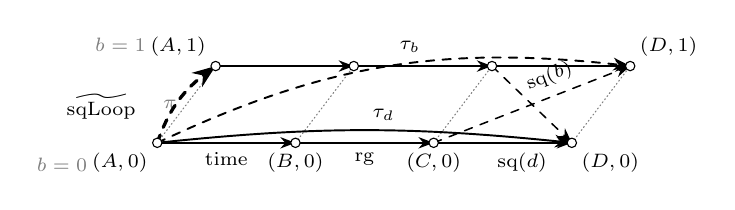
\begin{tikzpicture}[>=Stealth, line cap=round, line join=round, scale=0.78]
\def\dx{0.95}
\def\dy{1.25}
\tikzset{
  pt/.style={circle, draw, fill=white, inner sep=1.2pt},
  w0/.style={->, line width=0.55pt},
  w1/.style={->, dashed, line width=0.55pt},
  lift/.style={->, dashed, very thick},
  faint/.style={densely dotted, gray, line width=0.4pt},
  lab/.style={font=\scriptsize},
}

\coordinate (A0) at (0,0);
\coordinate (B0) at (2.25,0);
\coordinate (C0) at (4.50,0);
\coordinate (D0) at (6.75,0);

\coordinate (A1) at ($(A0)+(\dx,\dy)$);
\coordinate (B1) at ($(B0)+(\dx,\dy)$);
\coordinate (C1) at ($(C0)+(\dx,\dy)$);
\coordinate (D1) at ($(D0)+(\dx,\dy)$);

\draw[faint] (A0)--(A1) node[midway, left, lab, text=gray] {$\pi$};
\draw[faint] (B0)--(B1);
\draw[faint] (C0)--(C1);
\draw[faint] (D0)--(D1);

\node[lab, text=gray] at ($(A0)+(-1.55,-0.35)$) {$b=0$};
\node[lab, text=gray] at ($(A1)+(-1.55,+0.35)$) {$b=1$};

\draw[w0] (A0)-- node[lab, below] {$\mathrm{time}$} (B0);
\draw[w0] (B0)-- node[lab, below] {$\mathrm{rg}$} (C0);
\draw[w0] (A1)-- (B1);
\draw[w0] (B1)-- (C1);

\draw[w0] (C0)-- node[lab, below, pos=0.60, xshift=2pt] {$\mathrm{sq}(d)$} (D0);
\draw[w0] (C1)-- (D1);

\draw[w1] (C0)-- node[lab, above, sloped, pos=0.60, xshift=2pt] {$\mathrm{sq}(b)$} (D1);
\draw[w1] (C1)-- (D0);

\draw[->, line width=0.7pt] (A0) to[bend left=6] node[lab, above, pos=0.55] {$\tau_d$} (D0);
\draw[->, dashed, line width=0.7pt] (A0) to[bend left=16] node[lab, above, pos=0.55] {$\tau_b$} (D1);
\draw[lift, bend left=18] (A0) to node[lab, left, pos=0.4, xshift=-10pt] {$\widetilde{\mathrm{sqLoop}}$} (A1);

\node[pt] at (A0) {}; \node[lab, below left] at (A0) {$(A,0)$};
\node[pt] at (B0) {}; \node[lab, below]      at (B0) {$(B,0)$};
\node[pt] at (C0) {}; \node[lab, below]      at (C0) {$(C,0)$};
\node[pt] at (D0) {}; \node[lab, below right]      at (D0) {$(D,0)$};

\node[pt] at (A1) {}; \node[lab, above left] at (A1) {$(A,1)$};
\node[pt] at (B1) {};
\node[pt] at (C1) {};
\node[pt] at (D1) {}; \node[lab, above right]      at (D1) {$(D,1)$};
\end{tikzpicture}
\end{minipage}
\caption{(a) The two-time square commutes on record endpoints: $D=T_t(R_u(A))=R_u(T_t(A))$. (b) Lift to the $\Ztwo$-cover: $(X,b)$ denotes the lift of the same record endpoint $X\in\{A,B,C,D\}$ to sheet $b\in\Ztwo$, and dotted verticals indicate the projection $\pi$. Solid arrows have $\omega=0$ and preserve the sheet; dashed arrows have $\omega=1$ and flip sheets. The two completed corner procedures from $(A,0)$ land at different lifts of the same record endpoint, and the lifted square-loop $\widetilde{\mathrm{sqLoop}}$ is the monodromy from $(A,0)$ to $(A,1)$. Abbreviations: $\tau_d=\mathrm{toCorner}_{\mathrm{diag}}$, $\tau_b=\mathrm{toCorner}_{\mathrm{bridge}}$, $d=\mathrm{diag}$, $b=\mathrm{bridge}$.}
\label{fig:two-time-square}
\end{figure*}


\paragraph{Minimal formal model (compressed).}
We formalize the record/micro distinction by a record sector $\Sys$, a microscopic sector $\SK$,
and a diagonal embedding $\diag:\Sys\to\SK$ whose image is interpreted as record-classical microstates.
There is an involution $\swap:\SK\to\SK$ commuting with $\diag$.
Physical time is modeled by a group action $\actT:\Time\times\SK\to\SK$,
and RG/coarse-graining by a monoid action $\actU:\RG\times\SK\to\SK$ (with $\RG=\mathbb{N}$),
with weak commutation on $\SK$:
\begin{equation}
\actU(u,\actT(t,x))=\actT(t,\actU(u,x)).
\label{eq:weak-comm}
\end{equation}
One key modeling ingredient is \emph{strict diagonalization}: for each $u\ge 1$ there exists
$\Pi_u:\SK\to\Sys$ such that
\begin{equation}
\actU(u,x)=\diag(\Pi_u(x)).
\label{eq:diag}
\end{equation}
Fix a reference scale $u_\star=1$ and a section $\mathrm{sec}_\Pi:\Sys\to\SK$ with $\Pi_1(\mathrm{sec}_\Pi(r))=r$.
Record reflection holds: $\diag(r)=\diag(r')\Rightarrow r=r'$.
Finally, to encode two-time descent compatibility we assume a bisimplicial set $\CSK_{m,n}$
with commuting horizontal/vertical face maps; this yields bicomplex identities (below).
Full assumptions and their provenance in the Agda development are listed in the Supplemental Material \cite{SM}.
The cohomological core is machine-checked in Agda; the Supplemental Material includes an audit table mapping statements to modules/symbols.

\paragraph{Schwinger--Keldysh interpretation of $\SK$ and $\swap$.}
In the Schwinger--Keldysh / closed-time-path formalism for nonequilibrium quantum dynamics, one doubles the degrees of freedom by introducing forward/backward time branches \cite{Schwinger1961,Keldysh1965,Chou1985,Kamenev2011}.
This doubling carries a natural involution swapping branches.
We abstract this as an involution $\swap:\SK\to\SK$ satisfying $\swap\circ\diag=\diag$; in an operator instantiation it acts as transpose (or conjugation) in a preferred pointer basis.

\paragraph{Records as diagonal states.}
The record sector $\Sys$ is intended as the Universe’s classical ledger.
In a Hilbert-space instantiation, $\SK$ may be taken as a specified class of density operators and $\diag$ as the embedding of those density operators diagonal in the pointer basis \cite{Zurek1981PointerBasis,JoosZeh1985Emergence}.
The strict diagonalization axiom \eqref{eq:diag} says that any positive RG step lands in this diagonal subspace: coarse-graining erases off-diagonal micro-information while preserving record content.

\paragraph{Roadmap.}
(i) We derive record-level actions $T_t$ and $R_u$ and record-level closure of the square.
(ii) We define a presented groupoid of record procedures in which the square admits two canonical fillers.
(iii) The parity cocycle $\omega$ detects an intrinsic $\Ztwo$ holonomy and obstructs any endpoint-only relabeling (non-splitting).
(iv) Independently, two-time descent data yield bicomplex identities $Q_t^2=Q_u^2=\{Q_t,Q_u\}=0$.
(v) In the concrete instantiation, a detector makes the holonomy operational on $\Diff$.

\paragraph{Methods and proof structure.}
We use an axiomatic HoTT/presentational style (generators/relations for procedures and a parity cocycle), not cubical type theory; in particular we avoid interval primitives that could smuggle a built-in $\Ztwo$ via endpoints.
The cohomological core (procedure groupoid, $\omega$, $\Ztwo$-cover, non-splitting, bicomplex identities) is machine-checked in Agda (audit in the Supplemental Material).
The detector and the resulting nontriviality on $\Diff$ are derived analytically in a Hilbert-space instantiation.

\paragraph{Record-level square (endpoints commute).}
The assumptions induce record-level maps $R_u:\Sys\to\Sys$ and $T_t:\Sys\to\Sys$
(definitions in the Supplemental Material) for which the square closes on records:
\[
R_u(T_t(r))=T_t(R_u(r)).
\]
The theorem is not about this equality; it is about procedures realizing it.
In particular, Fig.~\ref{fig:two-time-square} commutes on record endpoints while still supporting a nontrivial procedure-level bit.

\paragraph{Procedure-level square (completions versus endpoints).}
Record-level closure $R_u(T_t(r))=T_t(R_u(r))$ asserts only that the \emph{corner record} is well-defined; it does not yet specify a physical \emph{procedure} realizing that corner.
Indeed, an RG step strictly projects microscopic states to the diagonal record sector, so to compare the two orderings of time and RG as procedures one must also specify how the erased microscopic degrees of freedom are completed (re-glued) in a way consistent with the corner record.
We encode this completion datum by adjoining, for each square parameterized by $(t,u,r)$, a square filler
\[
\begin{aligned}
\mathrm{sq}(f;t,u,r)&: R_u(T_t(r)) \to T_t(R_u(r)),\\
f&\in\{\mathrm{diag},\mathrm{bridge}\},
\end{aligned}
\]
as a generator in the presented record-process groupoid.
Objects are records $r\in\Sys$, and morphisms are generated by $\mathrm{time}(t,r)$, $\mathrm{rg}(u,r)$, and the fillers, together with composition and inverses; we write composition left-to-right: $p\pcomp q$ means ``do $p$ then $q$.''\@
Relations include only the groupoid laws and the time/RG action laws; in particular, no relation in the presentation collapses the two filler tags.
The two tags label two \emph{canonical} completions distinguished by the intrinsic involution $\swap$ (see Fig.~\ref{fig:two-time-square}(b) and the Supplemental Material).

Given a filler choice $f$, the corresponding completed corner procedure is
\begin{equation}
\begin{aligned}
\mathrm{toCorner}_f(t,u,r)
:=\ &\mathrm{time}(t,r)\pcomp \mathrm{rg}(u,T_t(r)) \\
&\pcomp \mathrm{sq}(f;t,u,r) : r \to T_t(R_u(r)).
\end{aligned}
\label{eq:toCorner}
\end{equation}
The two completed corner procedures share the same record endpoints but are inequivalent as procedures; their mismatch is the \emph{square-loop}
\begin{equation}
\begin{aligned}
\mathrm{sqLoop}(t,u,r)
:=\ &\mathrm{toCorner}_{\mathrm{diag}}(t,u,r) \\
&\pcomp \mathrm{toCorner}_{\mathrm{bridge}}(t,u,r)^{-1} : r \to r.
\end{aligned}
\label{eq:sqLoop}
\end{equation}
The parity functor $\omega$ is the presentation-induced $\Ztwo$-character which is trivial on $\mathrm{time}$ and $\mathrm{rg}$ and sends the bridge filler to the nontrivial element; hence $\omega(\mathrm{toCorner}_{\mathrm{diag}})=0$, $\omega(\mathrm{toCorner}_{\mathrm{bridge}})=1$, and $\omega(\mathrm{sqLoop})=1$ (cf.\ Proposition~\ref{prop:corner-witness} and Corollary~\ref{cor:sqloop-odd}).
Importantly, the existence of this odd loop does \emph{not} contradict endpoint commutation: the square closes on record endpoints while carrying a genuine one-bit holonomy at the procedure level.

\begin{remark}[Canonical fillers and non-collapse]
The relations of the presented process groupoid include only the groupoid laws and the time/RG action laws.
Deliberately, there is \emph{no} relation identifying $\mathrm{sq}(\mathrm{diag};t,u,r)$ with
$\mathrm{sq}(\mathrm{bridge};t,u,r)$: collapsing the tags forces the parity cocycle to become trivial and the
$\Ztwo$-cover to split (see Supplemental Material). We emphasize that we single out two \emph{canonical} fillers;
additional completions, if present, would require extra structure beyond the axioms and are not used.
\end{remark}

\begin{lemma}[$\omega$ is well-defined]
\label{lem:omega-well-defined}
The parity assignment above respects the defining relations of the record-process presentation and therefore defines
a well-defined functor $\omega$ to $\Ztwo$.
\end{lemma}

\noindent\emph{Proof idea.}
The groupoid relations and the time/RG action relations are generated entirely by $\mathrm{time}$ and $\mathrm{rg}$,
which have parity $0$, and there is no relation that collapses the two square fillers. Full details are in the Supplemental Material. \qed

\begin{proposition}[Corner-path witness of the obstruction]
\label{prop:corner-witness}
For any $t\in\Time$, $u\in\RG$, and $r\in\Sys$, the two corner procedures in \eqref{eq:toCorner} have the same source and target but different parity:
\[
\begin{aligned}
\omega\big(\mathrm{toCorner}_{\mathrm{diag}}(t,u,r)\big)&=0,\\
\omega\big(\mathrm{toCorner}_{\mathrm{bridge}}(t,u,r)\big)&=1.
\end{aligned}
\]
\end{proposition}

\begin{lemma}[Splitting $\Leftrightarrow$ coboundary form]
\label{lem:split-cob-prl}
The $\Ztwo$-cover splits iff there exists a function $\sigma:\Sys\to\Ztwo$ such that
\[
\omega(p)=\sigma(\mathrm{src}(p))+\sigma(\mathrm{tgt}(p)) \pmod 2
\]
for every record process $p$.
\end{lemma}

\noindent\emph{Proof idea.}
A splitting chooses, for each record $r$, a lift $(r,\sigma(r))$ to the cover and forces the displayed parity constraint on lifted morphisms;
conversely, such a $\sigma$ defines a canonical lift. Full details are in the Supplemental Material. \qed

\begin{theorem}[Intrinsic $\Ztwo$ holonomy / non-splitting]
\label{thm:non-splitting-prl}
Assume $\Sys\neq\emptyset$. The induced $\Ztwo$-cover of the record-process groupoid does not split.
Equivalently, $\omega$ is not a coboundary in the sense of Lemma~\ref{lem:split-cob-prl}.
\end{theorem}

\noindent\emph{PRL proof sketch.}
If a splitting existed, Lemma~\ref{lem:split-cob-prl} would make $\omega(p)$ depend only on endpoints, so parallel procedures with the same endpoints would have equal parity.
Proposition~\ref{prop:corner-witness} exhibits two parallel corner procedures with the same endpoints but different parity, contradiction. \qed

\begin{corollary}[Square-loop is odd]
\label{cor:sqloop-odd}
For all $t,u,r$ one has $\omega(\mathrm{sqLoop}(t,u,r))=1$.
\end{corollary}

\begin{corollary}[$\omega$-oddness on abelian coefficients]
\label{cor:omega-odd-abelian-prl}
Let $G$ be an abelian group. The parity functor $\omega$ induces a canonical sign action on $G$ via
\[
\mathrm{act}^G_{\omega}(p)(x):=(-1)^{\omega(p)}x.
\]
Then for every $t,u,r$ and $x\in G$,
\[
\mathrm{act}^G_{\omega}\big(\mathrm{sqLoop}(t,u,r)\big)(x)=-x.
\]
\end{corollary}

\noindent\emph{Proof.}
By Corollary~\ref{cor:sqloop-odd}, $\omega(\mathrm{sqLoop})=1$. \qed

\paragraph{Why Corollary~\ref{cor:omega-odd-abelian-prl} matters.}
It is the minimal algebraic sign rule seeded by the one-bit holonomy: any abelian coefficient system acquires a canonical $\Ztwo$-grading,
and square-loops act by the nontrivial sign. This is the bridge from the obstruction statement to graded/odd structures downstream.

\paragraph{Two-time descent object $\CSK_{m,n}$.}
The bisimplicial set $\CSK_{m,n}$ abstracts two-time descent data: an $(m,n)$-simplex encodes a compatible patch with $m$ time-like and $n$ RG-like steps.
Horizontal and vertical face maps delete one step in the corresponding direction.
The simplicial identities together with the mixed commutation $d_i^H d_j^V=d_j^V d_i^H$ are the ``no mixed anomaly'' condition: boundaries in the two directions are compatible.

\paragraph{Bicomplex identities (minimal).}
From this bisimplicial data, set $C_{m,n}:=\mathbb Z[\CSK_{m,n}]$ and define
\begin{align}
Q_t([x])&:=\sum_{i=0}^{m+1}(-1)^i[d_i^H x], \\
Q_u([y])&:= {}\\
&\sum_{j=0}^{n+1}(-1)^{m+j}[d_j^V y],
\label{eq:QtQu}
\end{align}
where the factor $(-1)^m$ in $Q_u$ is the Koszul twist by horizontal degree. Then
\begin{equation}
\begin{aligned}
Q_t^2&=0,\qquad Q_u^2=0,\\
Q_tQ_u+Q_uQ_t&=0,
\end{aligned}
\label{eq:bicomplex}
\end{equation}
by cancellations using the simplicial face identities and the mixed commutation $d_i^H d_j^V=d_j^V d_i^H$.

\begin{corollary}[Total boundary (``boundary of boundary is zero'')]
Let $Q:=Q_t+Q_u$ on the total complex $\bigoplus_{m,n}C_{m,n}$. Then $Q^2=0$.
\end{corollary}

\noindent\emph{Proof.}
Expand $Q^2=Q_t^2+(Q_tQ_u+Q_uQ_t)+Q_u^2$ and apply \eqref{eq:bicomplex}. \qed

\paragraph{Operational meaning via $\Diff$.}
Define the set-level cofiber $\Diff:=\Cofib(\diag)$, which collapses all diagonal record states to a basepoint and retains
precisely the information invisible to records. The involution $\swap$ induces $\flip:\Diff\to\Diff$.
In the Supplemental Material we construct a canonical action of record procedures on $\Diff$ in which the two filler tags act by
$\mathrm{diag}\mapsto \mathrm{id}_\Diff$ and $\mathrm{bridge}\mapsto \flip$.
Consequently a general process $p$ acts as $\flip$ exactly when $\omega(p)=1$, and square-loops act by $\flip$.

\paragraph{Detectability (mixing produces off-diagonal microdata).}
In the Hilbert-space instantiation (pointer basis; $\swap$ is transpose in that basis; unitary micro-evolution
$\rho(t)=e^{-itH}\rho e^{itH}$; and a mild mixing/nondegeneracy condition), one can exhibit a swap-odd detector.

\begin{proposition}[Derived detector (swap-odd and constant on records)]
\label{prop:detector}
There exist indices $a\ne b$ and a bounded self-adjoint observable
\[
O_{ab}:= i\big(\lvert a\rangle\langle b\rvert-\lvert b\rangle\langle a\rvert\big)
\]
such that $\obs_{ab}(\rho):=\mathrm{Tr}(\rho\,O_{ab})$ vanishes on every diagonal (record) state in the pointer basis and satisfies
$\obs_{ab}(\swap\rho)=-\obs_{ab}(\rho)$, yet for some time-evolved state $\rho(t)$ one has $\obs_{ab}(\rho(t))\ne 0$.
In particular, some intermediate microscopic states are off-diagonal, and $\flip$ has a non-fixed point on $\Diff$.
\end{proposition}

\noindent\emph{Proof sketch.}
Compute $\obs_{ab}(\rho)=i(\rho_{ba}-\rho_{ab})=2\,\Im(\rho_{ab})$.
If $\rho$ is diagonal in the pointer basis then $\rho_{ab}=0$ for $a\ne b$, hence $\obs_{ab}(\rho)=0$.
If $\swap$ is transpose in the pointer basis, then for Hermitian $\rho$ one has $(\swap\rho)_{ab}=\rho_{ba}=\overline{\rho_{ab}}$,
so $\Im((\swap\rho)_{ab})=-\Im(\rho_{ab})$ and $\obs_{ab}(\swap\rho)=-\obs_{ab}(\rho)$.
For $\rho(t)=e^{-itH}\rho e^{itH}$ with diagonal $\rho=\sum_c p_c\lvert c\rangle\langle c\rvert$, differentiation at $t=0$ gives
$\dot{\rho}_{ab}(0)=-iH_{ab}(p_b-p_a)$ and hence $\frac{d}{dt}\Im(\rho_{ab}(t))\rvert_{t=0}=-(p_b-p_a)\Re(H_{ab})$.
The mixing/nondegeneracy hypothesis supplies $p_a\ne p_b$ and $\Re(H_{ab})\ne 0$, so $\obs_{ab}(\rho(t))\ne 0$ for small $t$. \qed

\noindent
Consequently, the two fillers act differently on $\Diff$ and are operationally distinguishable (full derivation in the Supplemental Material).

\begin{theorem}[Two-Time Limited-Scope Theorem (2T-LS)]
\label{thm:2tls-package}
Under the assumptions of this Letter, the classical ledger sector inside reversible microscopic dynamics induces a limited-scope package with four components:
\begin{enumerate}
\item intrinsic $\Ztwo$ holonomy of record procedures, equivalently non-splitting of the induced $\Ztwo$-cover (Theorem~\ref{thm:non-splitting-prl});
\item canonical $\Ztwo$-gradedness together with the cochain-level total-boundary identity $Q^2=0$ following from Eq.~\eqref{eq:bicomplex};
\item for every abelian group $G$, the induced $\omega$-action is canonical and square-loops act by the nontrivial sign, i.e. by $x\mapsto -x$ (Corollary~\ref{cor:omega-odd-abelian-prl});
\item under the mixing/nondegeneracy hypothesis of Proposition~\ref{prop:detector}, operational detectability of that distinction on $\Diff$.
\end{enumerate}
\end{theorem}

\noindent\emph{Package status.}
The name ``2T-LS'' refers to this package of cohomological results together with its detector-based semantic add-on, not to a claim stronger than the individual results cited above.

\paragraph{From the thought experiment to the square-loop (SK/dilation semantics).}
In a Hilbert-space instantiation with pointer basis $\{\lvert a\rangle\}$, record states are diagonal and a reference forgetting step may be taken as strict diagonalization
$\Delta(\rho)=\sum_a \lvert a\rangle\langle a\rvert\,\rho\,\lvert a\rangle\langle a\rvert$.
The Schwinger--Keldysh involution $\swap$ swaps the two branches; in the operator model $\swap(\rho)=\rho^{\mathsf T}$ and $\swap\circ\diag=\diag$.
Because forgetting discards microscopic data, a boundary route becomes a procedure only after choosing a completion/gluing of erased degrees; the two filler tags encode two canonical choices, inducing $\mathrm{id}_\Diff$ (diag) and $\flip$ (bridge) on $\Diff=\Cofib(\diag)$ (Supplemental Material).
Transporting the completion across a reversible segment inserts the branch swap exactly once, so the mismatch $\mathrm{toCorner}_{\mathrm{diag}}\pcomp \mathrm{toCorner}_{\mathrm{bridge}}^{-1}$ is the square-loop $\mathrm{sqLoop}$ (Eq.~\ref{eq:sqLoop}) acting by $\flip$, and Proposition~\ref{prop:detector} supplies a non-fixed point to detect it.

\begin{corollary}[Three-checkpoint loop witness]
\label{cor:groundhog-loop}
If the thought-experiment checkpoint $A$ satisfies
\[
R_u(T_t(A))=T_t(R_u(A))=A,
\]
then
\[
\begin{aligned}
\omega\big(\mathrm{toCorner}_{\mathrm{diag}}(t,u,A)\big)&=0,\\
\omega\big(\mathrm{toCorner}_{\mathrm{bridge}}(t,u,A)\big)&=1.
\end{aligned}
\]
Thus even with identical initial and final record, ``forgetting after'' and ``forgetting before'' are distinct based loops at $A$; the one-bit distinction cannot be reduced to a label on record states.
\end{corollary}

\noindent\emph{Proof.}
This is Proposition~\ref{prop:corner-witness} specialized to the closed three-checkpoint case $R_u(T_t(A))=T_t(R_u(A))=A$. \qed

\paragraph{Discussion: theorem-level ``It from bit'' (interpretation and outlook).}
Wheeler’s slogan “It from bit” \cite{Wheeler1990ItFromBit} suggests that physics may ultimately be organized by information-theoretic primitives.
The present work provides a sharp form of this idea: under the assumption that the Universe admits a classical ledger of records
with a strict RG projection, the induced two-time structure yields both a canonical $\mathbb Z_2$-gradedness of procedures and,
via Eq.~\ref{eq:bicomplex}, a cochain-level total boundary $Q=Q_t+Q_u$ with $Q^2=0$. The same structure also produces an unavoidable
one-bit distinction between two procedures that are otherwise identical at the level of record endpoints.

Related work on 2T-physics introduces an additional timelike dimension and an Sp$(2,\mathbb R)$ gauge symmetry that yields families of 1T ``shadows'' \cite{Bars1998TwoTime,Bars2000TwoTimeField,Bars2008Gravity}.
Our ``two-time'' refers instead to physical time and RG/coarse-graining; we cite this literature to situate the term while the mechanisms and observables are distinct.

This is an \emph{objective arrow of time} in the precise theorem-backed sense relevant here. At cochain level, the two directions enter symmetrically through the bicomplex identities \eqref{eq:bicomplex}; at process level, $\omega$ is trivial on the pure time and pure RG generators, while square-loops are odd (Corollary~\ref{cor:sqloop-odd}). Thus neither time by itself carries the before/after bit.


Corollary~\ref{cor:groundhog-loop} shows that the bit appears only in their ordered interaction: even when the three-checkpoint loop closes on the same record $A$, ``forget-after'' and ``forget-before'' remain inequivalent based loops with different $\mathbb Z_2$ labels. Hence there exists no global assignment
of a $\mathbb Z_2$-label to record states that trivializes the distinction. 

It can be concluded therefore that, in a ledger-containing Universe, the \emph{procedure - mediated} \(\mathbb{Z}_2\) lift of the observable history defines ``before'' and ``after'' in a common meaning of ``becoming time''. In that precise sense, the human intuition of the multi-variant future
from which a choice is somehow being made highlighted by the thought experiment, that leads to the past/future distinction perception, acquires theorem-backed content.

\paragraph{Outlook.}In related 2T Main Theorem work, we use the resulting $\mathbb Z_2$-gradedness as input to graded algebraic structures and their
symmetry constraints. The conceptual message of the thought experiment is therefore not merely rhetorical: the minimal, universally accessible
distinction between before and after can serve as the seed for rigid structural consequences once a record sector and two-time interaction are present.

\begin{thebibliography}{99}
\bibitem{SM}
See Supplemental Material at [URL will be inserted by publisher] for full assumptions, proof details, the Agda audit table, and supporting derivations.

\bibitem{Schwinger1961}
J.~Schwinger, J.\ Math.\ Phys.\ \textbf{2}, 407 (1961), doi:10.1063/1.1703727.

\bibitem{Keldysh1965}
L.~V.~Keldysh, Sov.\ Phys.\ JETP \textbf{20}, 1018 (1965).

\bibitem{Chou1985}
K.-C.~Chou, Z.-B.~Su, B.-L.~Hao, and L.~Yu, Phys.\ Rep.\ \textbf{118}, 1 (1985).

\bibitem{Kamenev2011}
A.~Kamenev, \emph{Field Theory of Non-Equilibrium Systems} (Cambridge University Press, Cambridge, 2011).

\bibitem{Zurek1981PointerBasis}
W.~H.~Zurek, Phys.\ Rev.\ D \textbf{24}, 1516 (1981), doi:10.1103/PhysRevD.24.1516.

\bibitem{JoosZeh1985Emergence}
E.~Joos and H.~D.~Zeh, Z.\ Phys.\ B \textbf{59}, 223 (1985), doi:10.1007/BF01725541.

\bibitem{Wheeler1990ItFromBit}
J.~A.~Wheeler, in \emph{Complexity, Entropy, and the Physics of Information}, edited by W.~H.~Zurek (Addison-Wesley, Redwood City, CA, 1990).

\bibitem{Zurek2003Decoherence}
W.~H.~Zurek, Rev.\ Mod.\ Phys.\ \textbf{75}, 715 (2003), doi:10.1103/RevModPhys.75.715.

\bibitem{Brown2006TopologyGroupoids}
R.~Brown, \emph{Topology and Groupoids} (www.groupoids.org, Deganwy, United Kingdom, 2006).

\bibitem{Bars1998TwoTime}
I.~Bars, Two-Time Physics, arXiv:hep-th/9809034.

\bibitem{Bars2000TwoTimeField}
I.~Bars, Phys.\ Rev.\ D \textbf{62}, 046007 (2000), doi:10.1103/PhysRevD.62.046007.

\bibitem{Bars2008Gravity}
I.~Bars, Phys.\ Rev.\ D \textbf{77}, 125027 (2008), doi:10.1103/PhysRevD.77.125027.
\end{thebibliography}

\end{document}
